\PassOptionsToPackage{hyphens}{url}
\documentclass[a4paper,fleqn]{cas-dc}
\usepackage[authoryear,longnamesfirst]{natbib}
\usepackage{amsmath,amssymb,booktabs,array}
\usepackage{graphicx}

% cas-common sets the keywords box into a zero-width hbox without \hss, which TeX reports as a
% 123.6 pt overfull box at \maketitle. Same environment with \hss added: identical output.
\ExplSyntaxOn
\RenewDocumentEnvironment { Abstract } { o }
{
  \group_begin:
  \IfNoValueTF { #1 } { }
  { \tex_gdef:D \abstractname { #1 } }
  \parindent \c_zero_dim
  \box_if_empty:NTF \g_stm_key_box
  { \leftskip = .35 \textwidth }
  {
    \dim_gset:Nn \l_tmpa_dim { \box_ht:N \g_stm_key_box }
    \dim_gadd:Nn \l_tmpa_dim { \box_dp:N \g_stm_key_box }
    \leftskip .35\textwidth
    \hspace*{-.35 \textwidth }
    \noindent\hbox_to_wd:nn { \c_zero_dim } { \box \g_stm_key_box \hss }
    \skip_vertical:n { - \l_tmpa_dim }
  }
  \noindent \abstractname \par
  \skip_vertical:n { -4pt}
  \noindent \rule{.65\textwidth}{.2pt}\par \footnotesize
  \ignorespaces \everypar { \parindent=1.5em }
}
{ \par \group_end: }

% cas-common hard-codes "Preprint submitted to Elsevier" in the footer. This is an SSRN working
% paper, not an Elsevier submission, so the footer names the version instead.
\cs_set:Npn \__first_footerline:
{
  \group_begin:
  \small
  \sffamily
  \ifnum\theblind>0\relax
  \else
    \__short_authors: :~
  \fi
  { \rmfamily \itshape Working~paper,~\today }
  \group_end:
}
\ExplSyntaxOff

\begin{document}

\shorttitle{Who trades against the maker?}
\shortauthors{G. Albiez}

\title[mode=title]{Who trades against the maker? Adverse selection with counterparty identity on an on-chain options order book}

\author[1]{Gregor Albiez}[orcid=0009-0006-6036-4932]
\ead{gregor.albiez@students.fhnw.ch}
\affiliation[1]{organization={University of Applied Sciences and Arts Northwestern Switzerland (FHNW)},
                country={Switzerland}}

\begin{abstract}
Placeholder abstract. The manuscript is written in plan 5; this skeleton only proves that the
toolchain builds the CAS class with our figures.
\end{abstract}

\begin{keywords}
market microstructure \sep options \sep adverse selection \sep decentralised exchange \sep market making
\end{keywords}

\maketitle

\section{Placeholder}
Figure~\ref{fig:placeholder} is a placeholder that will be replaced in plan 4.

\begin{figure}[t]
  \centering
  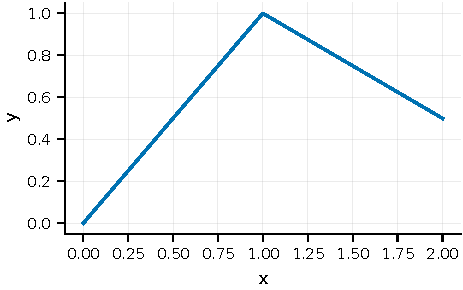
\includegraphics[width=\linewidth]{figures/placeholder.pdf}
  \caption{Placeholder figure produced by \texttt{derive\_surface.figstyle}.}
  \label{fig:placeholder}
\end{figure}

\bibliographystyle{cas-model2-names}
\bibliography{refs}

\end{document}
